\section{The declared delay-only comparator}\label{sec:delay}
The uniform law answers an orientation question, but it cannot answer whether a higher or more distant observer records a source earlier. SRG-04 therefore declares a second mathematical interface. It uses the same contacts, normals and observer frames, with a prescribed readout history and Euclidean delays. The distances supply arguments of a signal; they are not paths constrained to the red circle or material rays passing through panels.

For one readout $v$, write $W(t)=Av(t)$ and suppose its values are given at every retarded time needed below. No interpolation of native samples is implicit. An interpolation would require a separately chosen map $n\mapsto t_n$ and rule between samples; the native iteration $n$, supplied readout clock $(q,N,t_c)$, and analysis time $t$ remain distinct. Use contact index $\eta=(j,\sigma)$ when it avoids confusing the six labels with the scalar $a$.

\begin{definition}[Six-contact unit-gain delay reconstruction]\label{def:delay}
For a declared $c_*>0$, let
\begin{equation}\label{eq:delaylaw}
\begin{aligned}
q_\eta(t)&=n_\eta\tr W(t),&
d_\eta(X)&=\norm{X-P_\eta},&\tau_\eta(X)&=d_\eta(X)/c_*,\\
F(X,t)&=G^{-1}\sum_\eta n_\eta q_\eta(t-\tau_\eta(X)),&
Y_{mk}(t)&=B_{mk}\tr F(c_{mk},t).
\end{aligned}
\end{equation}
Here $G$ is exactly \eqref{eq:patchgram}. The histories for $M$ and $\Ch$ are kept separate; $T$ is their fixed linear blend.
\end{definition}
This definition has unit path gains and no spreading, blocking, damping, refraction or backreaction. It is an explicitly conditional comparison law from SRG-04, not a native propagation equation.~\cite[Eqn.~(3)]{SRG04} It has no evolving shared field state whose value is sampled by all sensors. Constant, harmonic and onset inputs used here are prescribed signal controls, not native trajectories.

\begin{proposition}[Baseline and covariance]\label{prop:baseline}
For constant $W$, or when all delays are zero, $F=W$ and $Y_{mk}=B_{mk}\tr W$. Under a common Euclidean coordinate change $X'=UX+a_0$, $U$ orthogonal, transform positions likewise and $n'=Un$, $A'=UA$, $B'=UB$, $G'=UGU\tr$. Then $F'(X',t)=UF(X,t)$ and $Y'=Y$.
\end{proposition}
\begin{proof}
Without differential time arguments the reconstruction is $G^{-1}\sum n_\eta n_\eta\tr W=W$. Orthogonal transformations preserve distances. Also $(UGU\tr)^{-1}=UG^{-1}U\tr$, $q'_\eta=(Un_\eta)\tr UW=q_\eta$, and substitution gives $F'=UF$. Left multiplication by $(UB)\tr$ cancels $U$. This includes improper coordinate changes; keeping $G$ artificially diagonal after a general rotation would fail this proof.
\end{proof}

\begin{proposition}[Contact-onset half-value]\label{prop:half}
Let $W(t)=w_0\mathbf1_{t\ge0}$ with zero prehistory. At $X=P_\eta$, for $t>0$ smaller than every other contact's delay,
\begin{equation}\label{eq:half}
n_\eta\tr F(P_\eta,t)=\tfrac12 q_\eta(t).
\end{equation}
In particular, when $q_\eta\ne0$ the assigned source value is not an imposed Dirichlet value of the reconstructed field.
\end{proposition}
\begin{proof}
All six contacts are distinct, so the stated interval is nonempty. Only the zero-length self-channel has arrived. Its projected reconstruction is $(n_\eta\tr G^{-1}n_\eta)q_\eta$. From \eqref{eq:planes} and \eqref{eq:patchgram},
\[
n_\eta\tr G^{-1}n_\eta=\frac47\frac7{12}+\frac37\frac7{18}
=\frac13+\frac16=\frac12.
\]
Choose, for example, $w_0=n_\eta$ to obtain the nonzero discrepancy. This is a counterexample within the declared law, not an inconsistency requiring replacement of that law.
\end{proof}
One may evaluate $F$ on $\Gamma_j$ and project onto its tangent. At the two contacts these projections equal $-(n_j^+)\tr F$ and $(n_j^-)\tr F$ respectively, but generally not the original instantaneous $-q_j^+$ and $q_j^-$. The circle angle is still a spatial variable, not travel time.

\section{Transfer bounds and a controlled inverse}\label{sec:transfer}
For the formal harmonic input $W(t)=\Re(\widehat w e^{i\omega t})$, with real $\omega$, define
\begin{equation}\label{eq:transfer}
\mathbf K(X,\omega)=G^{-1}\sum_\eta n_\eta n_\eta\tr e^{-i\omega\tau_\eta(X)},
\qquad \widehat Y_{mk}=B_{mk}\tr\mathbf K(c_{mk},\omega)\widehat w.
\end{equation}
This is an exact substitution into \eqref{eq:delaylaw}, not numerical evolution. In particular $\mathbf K(X,0)=\Id_3$.

\begin{theorem}[Compression, remainder and low-frequency invertibility]\label{thm:compression}
At any fixed position with finite delays, let $V=N_\Delta G^{-1/2}$ and define
\[
\norm L_G:=\norm{G^{1/2}LG^{-1/2}}_2.
\]
Then $V^*V=\Id_3$ and
\begin{equation}\label{eq:compression}
G^{1/2}\mathbf K G^{-1/2}
=V^*\diag(e^{-i\omega\tau_\eta})V,\qquad \norm{\mathbf K}_G\le1.
\end{equation}
For a reference delay $\tau_0$, set $\delta_\eta=\tau_\eta-\tau_0$, $\Delta=\max_\eta|\delta_\eta|$ and
\[
D_\delta=G^{-1}\sum_\eta n_\eta n_\eta\tr\delta_\eta.
\]
There is an exact expansion
\begin{equation}\label{eq:taylor}
\mathbf K=e^{-i\omega\tau_0}(\Id_3-i\omega D_\delta+E_2),
\qquad \norm{E_2}_G\le\tfrac12\omega^2\Delta^2.
\end{equation}
Writing $s_{\min,G}$ for the minimum singular value of the conjugated operator,
\begin{equation}\label{eq:lowinverse}
s_{\min,G}(\mathbf K)\ge1-|\omega|\Delta.
\end{equation}
Thus $|\omega|\Delta<1$ suffices for invertibility. The midpoint $\tau_0=(\tau_{\max}+\tau_{\min})/2$ minimizes $\Delta$.
\end{theorem}
\begin{proof}
By the definition of $G$, $V^*V=G^{-1/2}N_\Delta\tr N_\Delta G^{-1/2}=\Id_3$. Direct multiplication yields \eqref{eq:compression}. The middle diagonal operator is unitary, and the isometry $V$ and its adjoint have norm one, proving the weighted contraction.

For real $x$, two integrations of the exponential derivative give
\[
e^{-ix}-1+ix=-x^2\int_0^1(1-u)e^{-iux}\,du,
\quad |e^{-ix}-1+ix|\le x^2/2.
\]
Apply this identity to each $x=\omega\delta_\eta$ and compress by $V^*,V$. The constant term becomes the identity, the linear term becomes $-i\omega G^{1/2}D_\delta G^{-1/2}$, and the diagonal remainder norm is at most $\omega^2\Delta^2/2$. Undoing the similarity gives \eqref{eq:taylor}. Notice also that $GD_\delta$ is real symmetric.

The first-order difference estimate $|e^{-ix}-1|\le|x|$, from one integration, gives
\[
\norm{e^{i\omega\tau_0}\mathbf K-\Id_3}_G\le|\omega|\Delta.
\]
For a unit vector $z$ in the conjugated coordinates, the reverse triangle inequality then gives a norm of its image at least $1-|\omega|\Delta$. Taking the infimum proves \eqref{eq:lowinverse}. Finally, any centre of the interval $[\tau_{\min},\tau_{\max}]$ has maximum distance to its endpoints at least half the interval length. The midpoint attains that value, proving its minimax property.
\end{proof}

The small quantity is differential phase $|\omega|\Delta$, not necessarily the common phase $|\omega\tau_0|$. If every delay is $\tau_0$, the law is exactly a common shift. In general the bound is in the $G$ norm; no unqualified Euclidean contraction or physical energy monotonicity follows. Even a bounded invertible transfer at each frequency does not by itself produce a causal, stable real-time inverse.

\section{Height, radius, symmetry and reception}\label{sec:timing}
\subsection{Distance derivatives and an earliest possible onset}
Let $X-O=R e_r(\phi)+h\ez$, and $\gamma_j=\pi/2+2\pi j/3$. Subtracting the contact coordinates gives
\begin{equation}\label{eq:distance}
d_{j\sigma}^2=R^2+a^2-2aR\cos(\phi-\gamma_j)+(h-\sigma a)^2.
\end{equation}
Away from $d_{j\sigma}=0$, differentiation yields
\begin{equation}\label{eq:derivatives}
\partial_h d_{j\sigma}=\frac{h-\sigma a}{d_{j\sigma}},\qquad
\partial_R d_{j\sigma}=\frac{R-a\cos(\phi-\gamma_j)}{d_{j\sigma}}.
\end{equation}
At fixed $R,\phi$, moving from height zero toward $a$ shortens each upper-contact distance and lengthens each lower-contact distance. Above $a$, both sets increase. If $R>a$, all six distances increase with radius. Without this hypothesis, horizontal motion toward a contact can shorten a distance, so there is no universal radius statement. Changing height and radius together would mix these effects; this is the reason for the separated controls.

\begin{proposition}[Onset and its detection qualification]\label{prop:onset}
For simultaneous causal contact inputs with zero prehistory, the geometrically earliest possible delay is
\begin{equation}\label{eq:onset}
\tau_{\min}(R,\phi,h)=\frac1{c_*}\sqrt{R^2+a^2-2aR\max_j\cos(\phi-\gamma_j)+(|h|-a)^2}.
\end{equation}
For a step input $W=w_0\mathbf1_{t\ge0}$, let $\mathcal A$ be the group of earliest tied contacts. Its full-vector contribution is zero exactly when $n_\eta\tr w_0=0$ for every $\eta\in\mathcal A$. An individual observed component can vanish even if the full vector is nonzero.
\end{proposition}
\begin{proof}
Minimizing \eqref{eq:distance} over $j$ selects the maximum cosine, and minimizing over the independent sign selects $(|h|-a)^2$. No channel can arrive earlier under the stipulated zero prehistory. Put $Q_{\mathcal A}:=\sum_{\eta\in\mathcal A}n_\eta n_\eta\tr$. The first step contribution is $G^{-1}Q_{\mathcal A}w_0$. Since $G$ is invertible, it vanishes iff $Q_{\mathcal A}w_0=0$. The quadratic form is
\[
w_0\tr Q_{\mathcal A}w_0=\sum_{\eta\in\mathcal A}(n_\eta\tr w_0)^2.
\]
Its vanishing is equivalent to every summand vanishing, proving the full-vector claim. A projection onto one frame vector can annihilate a nonzero vector, establishing the component qualification.
\end{proof}

At an aligned site $\phi=\gamma_0$, $c_*\tau_{\min}=\sqrt{(R-a)^2+(|h|-a)^2}$. For $R=3$, the H levels $h=\pm a$ have distance $2.594480\ldots$, while $h=0,\pm2a$ all have distance $2.625981\ldots$. The higher outer levels therefore lose the earlier-arrival advantage in this height-only comparison. The values do not promise a nonzero signal for every source, and an eternal harmonic has phases without a first-arrival time.

\subsection{Reflection and threefold covariance}
\begin{proposition}[Exact parity relations]\label{prop:parity}
For $S_z=\diag(1,1,-1)$,
\begin{equation}\label{eq:parity}
\mathbf K(R,\phi,-h;\omega)=S_z\mathbf K(R,\phi,h;\omega)S_z.
\end{equation}
If $S_z\widehat w=p\widehat w$, $p\in\{+1,-1\}$, the matched same-frame records obey
\[
\widehat Y_- =p\diag(1,-1,1)\widehat Y_+.
\]
For the rotation $Q=R_z(2\pi/3)$ about $O$,
\begin{equation}\label{eq:c3}
\mathbf K(O+Q(X-O),\omega)=Q\mathbf K(X,\omega)Q\tr.
\end{equation}
\end{proposition}
\begin{proof}
Reflection interchanges $P_j^+$ with $P_j^-$ and $n_j^+$ with $n_j^-$. Thus delays are permuted and the dyads transform by $S_z$. The diagonal $G$ commutes with $S_z$, giving \eqref{eq:parity}. It follows that $\widehat F_-=pS_z\widehat F_+$. From \eqref{eq:frames}, $B\tr S_z B=\diag(1,-1,1)$, which gives the local-frame relation. Horizontal source vectors have $p=+1$ and vertical vectors have $p=-1$; a general vector is the sum of its two parity parts. For $Q$, the same proof uses the cyclic permutation $j\mapsto j+1$, $n\mapsto Qn$, and $QG=GQ$.
\end{proof}
At $h=0$, \eqref{eq:parity} rules out horizontal/vertical off-block mixing. At angular indices separated by four sites, \eqref{eq:c3} gives identical local records for a vertical source; a general fixed source must be rotated correspondingly before identical records follow. These response symmetries do not repair the body-reflection failure of Proposition~\ref{prop:mirror}; they are statements about the declared frames and input law.

\section{A pure-delay component and a blind-frequency counterexample}\label{sec:aligned}
An aligned equatorial position separates signal delay from amplitude interference particularly clearly. Let $R>0$, $h=0$, $\phi=\gamma_0$. The two contacts of pair zero have distance $d_0$, and the other four have distance $d_1$, where
\begin{equation}\label{eq:twodist}
d_0=\sqrt{(R-a)^2+a^2},\quad
d_1=\sqrt{R^2+aR+2a^2},\quad e_i=e^{-i\omega d_i/c_*}.
\end{equation}

\begin{theorem}[Aligned decomposition and all-frequency inverse]\label{thm:aligned}
In the common orthonormal basis $(u_0,v_0,\ez)$,
\begin{equation}\label{eq:aligned}
\mathbf K=\diag\left(\frac{2e_0+e_1}{3},\ e_1,\ \frac{e_0+2e_1}{3}\right).
\end{equation}
The tangential component is exactly a unit-gain delay $d_1/c_*$. For every real $\omega$, this site is invertible with Euclidean minimum singular value at least $1/3$. Consequently every accepted equatorial R ring, which contains an aligned site and records all three frame components, has a stacked transfer of rank exactly three at every real frequency.
\end{theorem}
\begin{proof}
Pair zero contributes the dyad $(8/7)u_0u_0\tr+(6/7)\ez\ez\tr$ with phase $e_0$. The remaining two pairs have $\sum_{j=1,2}u_ju_j\tr=(1/2)u_0u_0\tr+(3/2)v_0v_0\tr$, so their sum contributes $(4/7)u_0u_0\tr+(12/7)v_0v_0\tr+(12/7)\ez\ez\tr$ with phase $e_1$. Multiplication by $G^{-1}$ gives \eqref{eq:aligned}. In particular $v_0$ is orthogonal to both nearest normals; its source signal cannot arrive through the nearer pair.

Since $|e_i|=1$, the reverse triangle inequality gives $|2e_0+e_1|\ge1$ and $|e_0+2e_1|\ge1$. The diagonal basis is orthonormal, so these bounds divided by three and $|e_1|=1$ are exactly the singular-value lower bounds. A full local frame is orthogonal and preserves invertibility. A stack containing this invertible three-row block has rank at least three and, because it maps a single $\C^3$ source, at most three.
\end{proof}

The radial and vertical gains have equal squared magnitude,
\begin{equation}\label{eq:gain}
|\mathbf K_{zz}|^2=\frac{5+4\cos[\omega(d_1-d_0)/c_*]}9\in[1/9,1].
\end{equation}
This follows by multiplying the corresponding phasor sum by its conjugate. Distance is not required to weaken the signal in a unit-gain law. The tangential delay increases with radius because $d_1'=(R+a/2)/d_1>0$, while its magnitude remains one. The vertical magnitude changes with differential phase, not a spreading factor.

\begin{table}[htbp]\centering
\caption{Accepted aligned R fixtures. Distances are in shell-width units; gain uses the one prescribed phase condition $\omega a/c_*=\pi/2$. Rounded entries are manuscript-local substitutions, not a parameter scan.}
\begin{tabular}{@{}rrrr@{}}\toprule
$R$ & $d_0$ & $d_1$ & $|\mathbf K_{zz}|^2$\\\midrule
2 & 1.645240 & 2.267142 & 0.225148\\
3 & 2.625981 & 3.247376 & 0.225732\\
4 & 3.617283 & 4.236859 & 0.227840\\\bottomrule
\end{tabular}\label{tab:radius}
\end{table}

\begin{proposition}[Off-ring axial blindness]\label{prop:axis}
At $X=O+h\ez$, with no admissible positive-radius observer ring implied, let
\[
d_\pm=\sqrt{a^2+(h\mp a)^2},\qquad \tau_\pm=d_\pm/c_*.
\]
Then
\begin{equation}\label{eq:axis}
\mathbf K_{\rm axis}=e^{-i\omega(\tau_++\tau_-)/2}
\cos\!\left(\frac{\omega(\tau_+-\tau_-)}2\right)\Id_3.
\end{equation}
At $h=0$ it is a common shift. At $h\ne0$ it vanishes at each odd-$\pi$ differential phase.
\end{proposition}
\begin{proof}
For either sign, $\sum_j n_j^\sigma(n_j^\sigma)\tr=G/2$: the mixed terms cancel because $\sum u_j=0$, and the horizontal and vertical terms each make half the full Gram matrix. Thus $\mathbf K=(e^{-i\omega\tau_+}+e^{-i\omega\tau_-})\Id_3/2$, which is \eqref{eq:axis}. The squared-distance difference is $-4ha$, so for $h\ne0$ the two delays differ. Choosing $\omega(\tau_+-\tau_-)=(2m+1)\pi$ gives zero. This diagnostic lies at $R=0$, outside the $R_m>0$ ring family.
\end{proof}

\begin{figure}[htbp]\centering
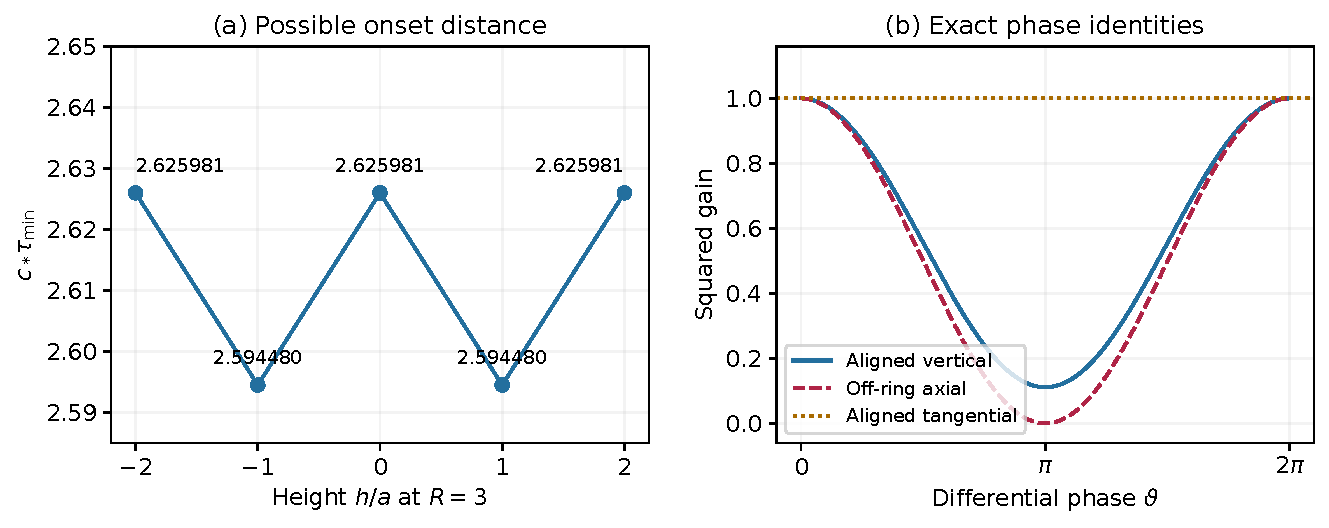
\includegraphics[width=\linewidth]{figures/delay_comparison.pdf}
\caption{Static reception comparison. Left: the accepted five-height nearest-distance values at the aligned $R=3$ site, divided by the symbolic $c_*$ to obtain possible arrival times. Right: analytic phase identities, with $\vartheta$ denoting differential phase. At aligned equatorial sites the squared vertical gain is $(5+4\cos\vartheta)/9$ and never vanishes; the tangential gain is one. At an off-ring axial point it is $\cos^2(\vartheta/2)$ and is zero at $\vartheta=\pi$. Curves sample closed formulas for drawing only; they are not time evolutions or a new frequency experiment.}\label{fig:delay}
\end{figure}

Theorem~\ref{thm:aligned} is therefore an aligned-site result, not a theorem for every point or every H family. Its validity depends on full-frame records; a scalar-only channel may still miss source components.

\section{Information and calibration in the delayed records}\label{sec:information}
At a fixed frequency, stack any finite collection of full-frame outputs for one source $\widehat w$. Every row factors through that same $\widehat w\in\C^3$, so the complex signal rank is at most three. The aligned R theorem supplies equality for those arrays. Additional sites can constrain a proposed transfer law, provide redundancy, or avoid a bad location without creating new coordinates of that source. The separate $M$ and $\Ch$ signals remain subject to their native/readout definitions; $T$ adds no independent input under a known blend.

A simultaneous delayed measurement depends on a history. It cannot inherit the instantaneous rank-four theorem by merely counting its outputs. If two prescribed state/readout histories have the same $I$ and $\Ch$ at every retarded argument and use the same supplied clock, their staged histories and all records of \eqref{eq:delaylaw} agree, by pointwise substitution. Pointwise common-phase changes leave those quantities unchanged while generally changing $J$. Whether both prescribed histories are trajectories of \eqref{eq:native}--\eqref{eq:sync} is a separate dynamical question, not established here. This is an exact statement about the observation operator, with no claim of native trajectory observability.

For a known nonzero tangential harmonic at two aligned equatorial sites, the ratio in the common $v_0$ component is
\begin{equation}\label{eq:aliases}
\frac{\widehat Y_2^{\rm tan}}{\widehat Y_1^{\rm tan}}
=\exp\!\left(-i\omega\frac{d_1(R_2)-d_1(R_1)}{c_*}\right).
\end{equation}
The common source phase cancels, but a single nonzero frequency determines reciprocal speed only modulo $2\pi/(\omega\Delta d_1)$, subject to positive-speed admissibility. This follows because adding that increment to $1/c_*$ changes the exponent by an integer multiple of $2\pi i$. Unknown site-clock offsets can produce the same phase difference. An unknown absolute length unit confounds length with speed; unknown frame or channel gains can confound extraction of the tangential component. Constant signals provide no speed information at all. Further frequencies or sites may constrain aliases, but uniqueness needs stated calibration and an admissible interval or phase-unwrapping condition. No speed is fitted here.

\section{An auxiliary delay-line storage balance}\label{sec:storage}
An ideal delay channel has a useful realization, provided its added state and initialization are named. For a real scalar input $q$, a length $d>0$ and the same $c_*>0$, take
\begin{equation}\label{eq:transport}
u_t+c_*u_\xi=0,\quad 0<\xi<d,\qquad u(0,t)=q(t).
\end{equation}
This one-way transport model is auxiliary to the signal law, not the shared periodic carrier considered in Paper II. Its coordinate $\xi$ is a line coordinate, not distance along $\Gamma_j$.

\begin{theorem}[Characteristics and model-defined storage]\label{thm:storage}
For $C^1$ input and compatible prehistory $u(\xi,0)=q(-\xi/c_*)$, the solution is $u(\xi,t)=q(t-\xi/c_*)$. The quadratic storage and its boundary balance are
\begin{equation}\label{eq:storage}
\begin{aligned}
E(t)&=\frac12\int_0^d u(\xi,t)^2\,d\xi
=\frac{c_*}{2}\int_{t-d/c_*}^{t}q(r)^2\,dr,\\
\dot E(t)&=\frac{c_*}{2}\big[q(t)^2-q(t-d/c_*)^2\big].
\end{aligned}
\end{equation}
For piecewise $C^1$ initial data $u_0$ with $u_0(0)=q(0)$, the characteristic solution before reaching the inlet is $u_0(\xi-c_*t)$, and after that it is $q(t-\xi/c_*)$. The boundary balance remains $\dot E=(c_*/2)[u(0,t)^2-u(d,t)^2]$ wherever the classical derivatives exist, and almost everywhere for the piecewise smooth solution. The delayed-input expression for the outlet holds only after the initial contents have left.
\end{theorem}
\begin{proof}
Along a line $\xi-c_*t=\text{constant}$, differentiation gives $d u/dt=u_t+c_*u_\xi=0$. Tracing backwards reaches either $(\xi-c_*t,0)$ or $(0,t-\xi/c_*)$, proving both characteristic formulas. For pure-delay prehistory they coincide. Substitution $r=t-\xi/c_*$ gives the second integral in \eqref{eq:storage}, and the fundamental theorem of calculus gives its derivative. Independently, multiplying \eqref{eq:transport} by $u$ and integrating yields
\[
\dot E=-c_*\int_0^d u u_\xi\,d\xi
=\frac{c_*}{2}[u(0,t)^2-u(d,t)^2],
\]
which also proves the arbitrary-initial-data balance. Piecewise smooth inputs, including a step with zero prehistory, are interpreted along characteristics; the integral balance remains valid and its derivative holds almost everywhere. At $d=0$ there is an immediate identity channel and zero storage.
\end{proof}

For a sustained real harmonic $q(t)=\Re(\widehat q e^{i\omega t})$, $\omega\ne0$, averaging $q^2$ over one period gives $|\widehat q|^2/2$. Thus mean storage is $d|\widehat q|^2/4$ and the two mean boundary rates are both $c_*|\widehat q|^2/4$. For constant real $q_0$, they instead are $dq_0^2/2$ and $c_*q_0^2/2$. These follow directly from \eqref{eq:storage}; no time integration is required.

The units are signal squared times length, with rates per analysis-time unit. Nothing identifies $E$ with a native Hamiltonian or physical energy emitted by the core. There is a decisive duplication limitation: adding an independent copy of the same delay channel leaves $q$ unchanged and adds another identical storage and boundary-rate term. Arbitrarily many independent sensor paths can therefore multiply the sum without debiting a shared source. The reconstruction weights in $F$ do not provide that debit. A shared-carrier model needs its own state, allocation or input operator, geometry and balance; closed reciprocal exchange would require backreaction as well. A one-way delay does not establish a returning or circulating path.
